% \begin{document}
\chapter{Probabilistic approach}
\section{core idea}
we have two main points of views:
\begin{itemize}
    \item \textbf{traditional view}: we wanna to approximate a function $f:X\to X$
    \item \textbf{Probabilist view}: we wanna compute probablilities: $p: P( Y\mid  X)$
\end{itemize}
\subsection{Probs basics}
\subsubsection{Random variables}
A random variables $X$ represents an oyt come about which we're ncertain
\ex{Random variables}{
\begin{itemize}
    \item $X=$\texttt{true} if a randomly drawn stdent is male
    \item $X=$ first name of the student
    \item $X=$\texttt{true} if a randomly drawn stdent have the same birthday
\end{itemize}
}
 
Formal def:
\dfn{Probs variables}{
    the set $\Omega$ of the possible outcomes is called the sample space. It is said random variable a measurable function over $\Omega$:
    \begin{itemize}
        \item Discrete: $\Omega \to \{m,f\}$
        \item Continuos: $\Omega\to \mathbb{R}$
    \end{itemize}
}
 
\dfn{Probs def}{
    it is defined $P(X)$ is the fraction of times $X$ is true in repeated runs of the same experiment.
}

\nt{
    The definition requires that all samples 
}

Pay attention:
\wc{
    bad examples
}{
    Sample space, let $\Omega$ be a space made the possibile sum:
    \[
        \Omega = \{2,3,4,\dots, 12\}
    \]
    Problem: not all sums are equally likely! It should be:
    \[
        \begin{array}{c}
            P(sum = 2) = 1/11\\
            P(sum = 7) = 1/11
        \end{array}
    \]
    but in reality:
    \begin{itemize}
        \item Sum = 2: can only happen one way: $(1,1)$
        \item Sum = 7: can happen six ways:$(1,6), (2,5), (3,4), (4,3), (5,2), (6,1)$
    \end{itemize}

    so 
    \[
        P(sum = 2) \neq P(sum = 7)
    \]
}

A correct approach is 
\clm{correct approach}{}{
    Be $\Omega = {(1,1), (1,2), (1,3), ..., (6,5), (6,6)}$, where $|\Omega|=36 $outcomes

    each pair has equally probability = $\frac{1}{36}$
    
    Now here is a correctly computing:
    \[
        \begin{array}{c}
            P(sum = 2) = \frac{|{(1,1)}|}{36} = \frac{1}{36}\\
            P(sum = 7) = \frac{|{(1,6), (2,5), (3,4), (4,3), (5,2), (6,1)}|}{36} = \frac{6}{36}
        \end{array}
    \]
}

\subsubsection{The Axioms of Probability Theory}
These are the fundamental rules that make probability a "reasonable theory of uncertainty":

\ax{Axioms of probability theory}{
    \begin{align}
        &\text{(1) Non-negativity: } && 0 \leq P(A) \leq 1 \quad \text{for all events } A. \\
        &\text{(2) Normalization: } && P(\Omega) = 1. \\
        &\text{(3) Countable additivity: } && 
        \text{If } A_1, A_2, \dots \text{ are disjoint, then } 
        P\!\left(\bigcup_{i=1}^\infty A_i\right) = \sum_{i=1}^\infty P(A_i).
    \end{align}
}

Then:

\cor{consequences of the axioms}{
\begin{itemize}
    \item Monotonicity: If $A \subseteq B$, then $P(A) \le P(B)$
    \item Union rule (for two events): $P(A \cup B) = P(A) + P(B) - P(A \cap B)$
    \item $P(True) = 1$
    \item $P(False) = 0$
\end{itemize}
}

\begin{center}
    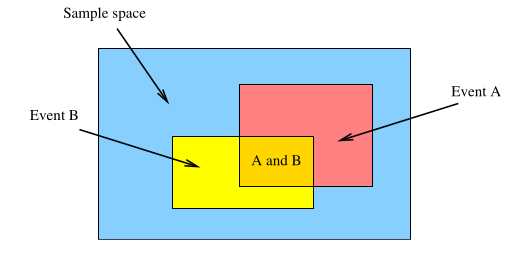
\includegraphics[width=5cm]{probs_ax.png}
\end{center}

\subsubsection{Derivied theorems}
\cor{Complement Rule
}{
    \[
        P(\lnot A) = 1- P(A)
    \]
}
\pf{Dm}{
\[
P(A \cup \neg A) = P(A) + P(\neg A) - P(A \cap \neg A)
\]

But: 
\[
P(A \cup \neg A) = P(\text{True}) = 1
\quad \text{and} \quad
P(A \cap \neg A) = P(\text{False}) = 0
\]

Therefore:
\[
1 = P(A) + P(\neg A) - 0
\quad \implies \quad
P(\neg A) = 1 - P(A) \qed
\]

}

\cor{Partition Rule}{
    \[
        P(A) = P(A \cap B) + P(A \cap \neg B)
    \]
}
\pf{Proof}{
    \[
\begin{aligned}
A &= A \cap (B \cup \neg B) &\text{[since $B \cup \neg B$ is always True]}\\
  &= (A \cap B) \cup (A \cap \neg B) &\text{[distributive law]}
\end{aligned}
\]

Hence,
\[
\begin{aligned}
P(A) &= P((A \cap B) \cup (A \cap \neg B)) \\
     &= P(A \cap B) + P(A \cap \neg B) - P((A \cap B) \cap (A \cap \neg B)) \\
     &= P(A \cap B) + P(A \cap \neg B) - P(\text{False}) \\
     &= P(A \cap B) + P(A \cap \neg B)
\end{aligned}
\]

}
\subsubsection{Multivalued Discrete Random Variables}
\dfn{
    k-value Discrete Random Variables
}{
    A random variable $A$ is \textit{$k$-valued discrete} if it takes exactly one value from 
    \[
    \{\nu_1, \nu_2, \dots, \nu_k\}.
    \]
}

\mprop{Key proprieties}{
    \begin{enumerate}
    \item \textbf{Mutual exclusivity:} For $i \neq j$,
    \[
        P(A = \nu_i \cap A = \nu_j) = 0
    \]

    \item \textbf{Exhaustiveness:}
    \[
        P(A = \nu_1 \cup A = \nu_2 \cup \dots \cup A = \nu_k) = 1
    \]
\end{enumerate}

}

\subsubsection{Conditional Probability}
\dfn{Conditional probs}{
    The Conditional probs of the event $A$ \textit{given} the event $B$ is defined as the quantity
    \begin{center}
        \begin{math}
            P(A\mid B) = \frac{P(A\cap B)}{P(B)}            
        \end{math}
    \end{center}
}

\cor{Cahin roule}{
    \[
        P(A\cap B) = P(B)P(A\mid  B)= P(A) P(B\mid A)
    \]
}
\subsubsection{Independent Events}
\dfn{Independent Events}{
    Events $A$ and $B$ are independent when:
    \begin{center}
        \begin{math}
            P(A\mid  B) = P(B)
        \end{math}
    \end{center}
}
(Meaning: B provides no information about A.)
\cor{consequences}{
    \begin{itemize}
        \item $P(A\cap b) = P(A)P(B)$ (from chail roule)
        \item $P(B|A) = P(B)$ (symmetry)
    \end{itemize}
}

\subsubsection{Bayes' Rule: The Heart of Probabilistic ML (ok chat... really?)}
\thm{Bayes's roule}{
    Now we have Bayes roule
    \begin{center}
        \begin{math}
            P(A\mid  B) = \frac{P(A)  P(B\mid A)}{P(B)}
        \end{math}
    \end{center}
}
\pf{Proof}{
    It's true by the chain roule that: $P(A \cap B) = P(B)  P(A\mid B)$. It's true also the reverse case $P(A \cap B) = P(B) · P(A\mid B)$.

    Since both expressions equal $P(A \mid B)$, they must equal each other:
    \[
        P(A)  P(B\mid A) = P(B)  P(A\mid B) 
    \]
    that it's equal to
    \[
        P(A\mid B) =\frac{[P(A)  P(B\mid A)]}{P(B)}
    \]
}
\ex{The trousers problem}{
    Setup:
    \begin{itemize}
        \item 60\% of students are boys, 40\% are girls
        \item girls wear in the same number skirt and trousers
        \item boys only wear trousers
    \end{itemize}
    If we see a student wearing trousers, what is the probability that is a girl?
}
\pf{Solution}{
    The probs a priori that a strudent is a girl is
    \[
        P(G) = \frac{2}{5}
    \]
    the probability that a student wears trousers is
    \[
        P(T) = \frac{1}{5} + \frac{3}{5} = \frac{4}{5}
    \]
    the probability that a student wear trousers, given that the student is a girl, is
    \[
        P(T\mid G) = 1/2
    \]
    So 
    \[
        P(G\mid T) =\frac{p(G)p(T\mid G)}{P(T)}=\frac{2/5\cdot 1/2}{4/5} = 1/4
    \]
}

\paragraph{Machine Learning Form}
\paragraph{Machine Learning Form}
For discrete $Y$ with values $\{y_1, y_2, \ldots, y_m\}$ and $X$ with values $\{x_1, x_2, \ldots, x_n\}$:
\[
P(Y = y_i \mid X = x_j) = \frac{P(Y = y_i) \cdot P(X = x_j \mid Y = y_i)}{P(X = x_j)}
\]

\textbf{Expanding the denominator:}
\begin{align*}
P(X = x_j) &= \sum_{i} P(X = x_j, Y = y_i) \quad \text{[sum over all $Y$ values]} \\
           &= \sum_{i} P(Y = y_i) \cdot P(X = x_j \mid Y = y_i) \quad \text{[chain rule]}
\end{align*}

\textbf{Complete Bayes' Rule:}
\[
P(Y = y_i \mid X = x_j) = \frac{P(Y = y_i) \cdot P(X = x_j \mid Y = y_i)}{\sum_{i} P(Y = y_i) \cdot P(X = x_j \mid Y = y_i)}
\]

\textbf{Terminology:}
\[
\underbrace{P(Y \mid X)}_{\text{posterior}} = \frac{\overbrace{P(X \mid Y)}^{\text{likelihood}} \cdot \overbrace{P(Y)}^{\text{prior}}}{\underbrace{P(X)}_{\text{marginal}}}
\]

\begin{itemize}
    \item \textbf{Posterior} $P(Y \mid X)$: What we want -- probability of $Y$ given observed $X$
    \item \textbf{Likelihood} $P(X \mid Y)$: How likely is $X$ if $Y$ is true?
    \item \textbf{Prior} $P(Y)$: What we believed before seeing $X$
    \item \textbf{Marginal} $P(X)$: Overall probability of observing $X$ (normalization constant)
\end{itemize}

\textbf{Alternative form:}
\[
\text{Posterior} = \frac{\text{Likelihood} \cdot \text{Prior}}{\text{Marginal Likelihood}}
\]
where:
\[
\text{Marginal} = \sum_{Y} P(X \mid Y) \cdot P(Y)
\]

The term ``marginal'' means we've \textbf{marginalized} (integrated/summed) over $Y$.

\section{The Joint Distribution}

\dfn{Joint Distribution}{
    Let $X_1, X_2,\dots, X_n$ be discrete random variables. The \textit{joint probability distribution} (or \textit{joint distribution}) of these variables is the function:
    \begin{center}
        \begin{math}
            P(X_1 = x_1, X_2 = x_2, \dots, X_n = x_n)
        \end{math}
    \end{center}

    which assigns to every possible combination of values \( (x_1, x_2, \dots, x_n) \) the probability that the random variables simultaneously take those values.

    Formally, for discrete variables, the joint distribution satisfies:
    \begin{itemize}
        \item \( 0 \leq P(x_1, x_2, \dots, x_n) \leq 1 \) for all \( (x_1, \dots, x_n) \)
        \item \( \sum_{x_1} \sum_{x_2} \cdots \sum_{x_n} P(x_1, x_2, \dots, x_n) = 1 \)
    \end{itemize}
}

Let's see an example
\ex{Joint distribution}{
    \begin{itemize}
        \item build a table with all possible combinations of values of random variables (features)
        \item compute the probability for any different combination of values
    \end{itemize}

    \begin{center}
        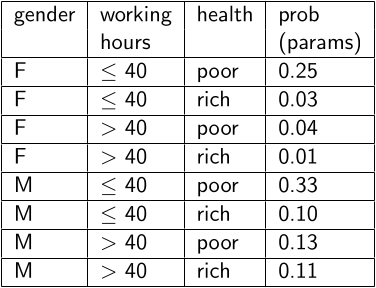
\includegraphics[width=6pt]{jd_img.png} % the table of the document
    \end{center}

    This table is the "Joint distribution"!

    Having that we may compute the probability of any event expressible as a logical combination of the features, with this formula
    \[
        P(E) = \sum_{row\in E} (row)
    \]
    in words for calculating an event we must add each row that is contained by the event. Let's provide an example (of an example)

        Let us compute the probability $P(M, poor)$
        \begin{center}
            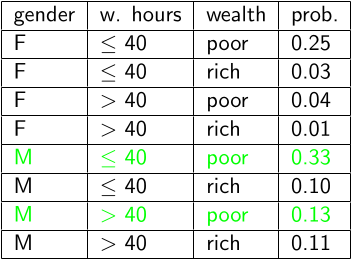
\includegraphics[width=6cm]{jd_ex.png}
        \end{center}
    

    we have: $P(M, poor) = 0.33 + 0.13 = 0.46$
}

\subsection{Inference with the Joint distribution}
Here are with the inference:
\dfn{Contintional probability}{
    Let \( E_1 \) and \( E_2 \) be two events defined as logical conditions over subsets of the random variables (e.g., \( E_1: X_i = a, X_j = b \); \( E_2: Y = y \))

    Then, \textit{conditional probability} of \( E_1 \) given \( E_2 \) is:
    \[
        P(E_1 \mid E_2) = \frac{P(E_1 \land E_2)}{P(E_2)} = 
        \frac{\displaystyle\sum_{{row} \in (E_1 \land E_2)} P({row})}
        {\displaystyle\sum_{{row} \in (E_2)} P({row})}
    \]
}

for instance:
\ex{Conditional probability}{
    Let's compute $P(M|poor ) =\frac{P(M \land poor)}{P(poor)}$. We know that $P(M, poor ) = 0.46$. Let us compute $P(poor )$:
    \begin{center}
        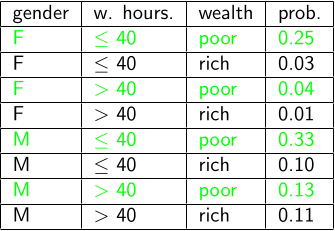
\includegraphics[width=6cm]{joint_inf.png}
    \end{center}
    Easy! $P(poor) = .75 \land P(M|poor) = 0.46/0.75 = 0.61$
}

\subsection{Complexity issues}
Let us build the joint table relative to
\[
    P(Y = wealth|X_1 = gender , X_2 = orelav.)
\]

\begin{center}
    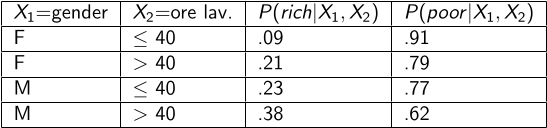
\includegraphics[width=6cm]{comp_issue.png}
\end{center}
To fill the table we need to compute $4=2^2$ parameters

If we have $n$ random variable $X = X_1 \times X_2 ,\dots, X_n$ where each $X_i$ is
boolean, we need to compute $2^n$ parameters. These parameters are \textit{probabilities}: to get reasonable value we would need a huge amount of data.

In particular the The Joint Distribution Requires \textit{Exponential parameters}
\ex{features and params}{
    \begin{itemize}
        \item With just 10 binary features, you need $2^{11}-1=2047$ parameters
        \item With 20 features: over 1 million parameters
        \item With 100 features: $2^{101}$ a number larger than the estimated atoms in the observable universe.
    \end{itemize}
}
This is computationally and statistically infeasible.
\subsubsection{USing Bayes}
for reducing complexity, we can rewrite the formula with the Bayes' rule:
\[
    P(Y=y_i\mid X=x_j) = \frac{P(Y=y_i)\cdot P(X = x_j\mid Y = y_i)}{\sum_i P(Y=y_i)\cdot P(X=x_j \mid Y=y_i)}
\]
generalising:
\[
    P(Y \mid X_1, X_2, \dots, X_n) = \frac{P(Y) \cdot P(X_1, X_2, \dots, X_n \mid Y)}{P(X_1, X_2, \dots, X_n)}
\]

But... there is a problem, it's required to know 
\[
    P(X_1, X_2, \dots, X_n \mid Y)
\]

that is the joint distribution of the features given $Y$, that requires, another time, $2^n$ params

\subsection{Naive Bayes}
For atteniung the complexity, it's possible assume an indipendencies conditional hypotesis, called "Naïve Bayes":
\[
    P(X_1,X_2,\dots,X_n|Y)=\prod_{i}P(X_i |Y)
\]
So given $Y$, $X_i$ and $X_j$ are independent from each other. In other therms:
\[
    P(X_i|X_j,Y)=P(X_i|Y)
\]
\nt{
    This means: onece we know $Y$, the feature $X_i \forall i$ are independents between each others
}
\ex{example 1}{
    A box contains two coins: a regular coin and a fake two-headed coin ($P(H) = 1$).Choose a coin at random, toss it twice and consider the following events:

    \begin{itemize}
        \item $A =$ First coin toss is H
        \item $B =$ Second coin toss is H
        \item $C =$ First coin is regular
    \end{itemize}
}
\ex{example 2}{
    For individuals, height and vocabulary are not independent, but they are if age is given.
}

\subsubsection{Giga formula with naive bayes}
\thm{Bayes rule}{
    \[
       P(Y = y_i \mid X_1, \dots, X_n) = \frac{P(Y = y_i) \cdot P(X_1, \dots, X_n \mid Y = y_i)}{P(X_1, \dots, X_n)}
    \]
}
\pf{Proof}{
    Left to mesco as exercice
}

\thm{Naïve Bayes}{
    \[
    P(Y = y_i \mid X_1, \dots, X_n) = \frac{P(Y = y_i) \cdot \prod_j P(X_j \mid Y = y_i)}{P(X_1, \dots, X_n)}
    \]
}
\pf{Proof}{
    Left to Bonzo as exercice
}

\thm{Classification of a new sample $x^{\text{new}} = \langle x_1, \dots, x_n \rangle$}{
    \label{thm:cne}
    Given a new instance represented by the feature vector $x^{\text{new}} = (x_1, x_2, \dots, x_n)$, 
    the predicted class is obtained as:
    \[
        Y^{\text{new}} = \arg\max_{y_i} \, P(Y = y_i) \cdot \prod_{j} P(X_j = x_j \mid Y = y_i)
    \]
}

\pf{Proof}{
  Seen as, using Bayes' formula, $ \forall i $ the denominator used to calculate $ P(Y = y_i | X_1, ..., X_n) $ remains the same,if we're only interested in maximizing the probability it's possible to only consider the numerator.

  Given $ P(X_1, ..., X_n) = C $, 
  \begin{align*}
    P(Y = y_i)\cdot \prod_{j}P(X_j | Y = y_i) &= C\cdot \frac{P(Y = y_i)\cdot \prod_{j}P(X_j | Y = y_i)}{C} \\
    &= C \cdot P(Y=y_i | X_1,...,X_n) \\
  \end{align*}

  Because $ C $ is a positive constant for each $ y_i $, $ arg max_{y_i} P(Y=y_i | X_1,...,X_n) = arg max_{y_i} C \cdot P(Y=y_i | X_1,...,X_n) $.
}

\nt{
    Theorem~\ref{thm:cne} expresses the decision rule of the Naïve Bayes classifier.
    Given a new vector of features $x^{\text{new}} = (x_1, x_2, \dots, x_n)$, 
    we estimate the most probable class $y_i$ by maximizing the posterior probability 
    $P(Y = y_i \mid X_1 = x_1, \dots, X_n = x_n)$, 
    which—under the conditional independence assumption—reduces to the product of the prior $P(Y = y_i)$ 
    and the individual likelihoods $P(X_j = x_j \mid Y = y_i)$.
}

\section{Learning algorithm}
Given discrete Random Variables $X_i, Y$, there are two phases
\begin{itemize}
    \item \textbf{Training}: in this phases the maching learn from the data of training set, estimating two types of probs:
    \begin{itemize}
        \item \textbf{Prior} (prob of the classes). For any possible value $y_k$ of $Y$ , estimate
        \[
            \pi_k = P(Y = y_k)
        \]
        example: if 9 out of 14 matches are "Play = Yes", then $\pi_{yes}= \frac{9}{14},\quad \pi_{no}= \frac{5}{14} $

        \item \textbf{Likelihoods}:(conditional probabilities of features). for any possible value $x_{ij}$ of $X_i$ estimate:
        \[
            \theta_{ijk} = P(X_i = x_{ij}\mid Y = y_k)
        \]
        It's the probability that a certain feature $X_i$ assumes the value $X_{ij}$, given $y_k$.

        example: $P(Outlook=Sunny\mid Play=Yes)=\frac{2}{9}$
    \end{itemize}
    \item \textbf{Classification of $a^{new} = \langle a_1 , \dots a_n \rangle$} (a vector with $n$ observed values (one for each feature)). We want to establish which class it belong to
    
    decision-making formula:
    \[
    \begin{aligned}
    Y^{\text{new}} &= \arg \max_{y_k} P(Y = y_{k}) \cdot \prod_{i} P(X_{i} = a_{i} \mid Y = y_{k}) \\
    &= \arg \max_{k} \pi_{k} \prod_{j} \theta_{ijk}
    \end{aligned}
    \]

    where:
    \begin{itemize}
        \item $P(Y=y_k)$: prior
        \item $P(X_i=a_i\mid Y=y_k)$: likelihood for each features
        \item the prod $\prod_{i}$ is given by Naive assumption
    \end{itemize}
\end{itemize}

\ex{a good day to play tennis?}{
    we wanna build a model that, given certain weather conditions, predict whether it is a good day to play tennis or not 
    
    Our class variable is:
    \[
        Y=Play\in\{Yes,No\}
    \]
    and the features observed are:
    \[
        X_1 = Outlook \quad X_2 = Temp \quad X_3=Humidity \quad X_4=Wind
    \]

    Here we have the dataset:
    \begin{table}[H]
\centering
\caption{Dataset for the \textit{Play Tennis} classification problem}
\label{tab:play_dataset}
\begin{tabular}{ccccc}
\toprule
Outlook & Temp & Humidity & Wind & Play \\
\midrule
Sunny & Hot & High & Weak & No \\
Sunny & Hot & High & Strong & No \\
Overcast & Hot & High & Weak & Yes \\
Rain & Mild & High & Weak & Yes \\
Rain & Cool & Normal & Strong & No \\
Overcast & Cool & Normal & Strong & Yes \\
Sunny & Mild & High & Weak & No \\
Sunny & Cool & Normal & Weak & Yes \\
Rain & Mild & Normal & Weak & Yes \\
Sunny & Mild & Normal & Strong & Yes \\
Overcast & Mild & High & Strong & Yes \\
Overcast & Hot & Normal & Weak & Yes \\
Rain & Mild & High & Strong & No \\
\bottomrule
\end{tabular}
\end{table}

TODO: TABELLA FATTA FARE DA UN LLM NON È VENUTA BENISSIMO

    \textbf{Calculating the prior}

    From the dataset we can compute the prior probabilities of the class variable $Y$:

    \[
    P(Y = \text{Yes}) = \frac{9}{14}, \qquad
    P(Y = \text{No}) = \frac{5}{14}.
    \]

    These represent the empirical frequencies of the two possible outcomes of $Y$.

    \medskip
    \textbf{Calculating the likelihoods}

    For each feature $X_i$ and each class $Y = y_k$, we estimate the conditional probabilities
    \[
    P(X_i = x_{ij} \mid Y = y_k),
    \]
    that is, the probability of observing a certain feature value $x_{ij}$ given that the class is $y_k$.

    For example:

    \[
    P(\text{Outlook} = \text{Sunny} \mid Y = \text{Yes}) = \frac{2}{9}, \qquad
    P(\text{Outlook} = \text{Sunny} \mid Y = \text{No}) = \frac{3}{5}.
    \]

    These values are computed as the relative frequencies in the dataset.

    \medskip
    \textbf{Classification of a new instance}

    Suppose we want to classify the new day
    \[
    x^{\text{new}} = (\text{Outlook} = \text{Sunny},\ 
    \text{Temp} = \text{Cool},\ 
    \text{Humidity} = \text{High},\ 
    \text{Wind} = \text{Strong}).
    \]

    We apply the Naïve Bayes decision rule:
    \[
    Y^{\text{new}} = 
    \arg\max_{y_i} P(Y = y_i) 
    \cdot 
    \prod_j P(X_j = x_j \mid Y = y_i).
    \]

    \medskip
    For $Y = \text{Yes}$:
    \[
    P(\text{Yes}) \cdot P(\text{Sunny}|\text{Yes}) \cdot P(\text{Cool}|\text{Yes}) 
    \cdot P(\text{High}|\text{Yes}) \cdot P(\text{Strong}|\text{Yes})
    = \frac{9}{14} \cdot \frac{2}{9} \cdot \frac{3}{9} \cdot \frac{3}{9} \cdot \frac{3}{9} 
    \approx 0.0053
    \]

    For $Y = \text{No}$:
    \[
    P(\text{No}) \cdot P(\text{Sunny}|\text{No}) \cdot P(\text{Cool}|\text{No}) 
    \cdot P(\text{High}|\text{No}) \cdot P(\text{Strong}|\text{No})
    = \frac{5}{14} \cdot \frac{3}{5} \cdot \frac{1}{5} \cdot \frac{4}{5} \cdot \frac{3}{5} 
    \approx 0.0205
    \]

    \medskip
    \textbf{Decision:}

    Since
    \[
    P(Y = \text{No} \mid x^{\text{new}}) > P(Y = \text{Yes} \mid x^{\text{new}}),
    \]
    the predicted class is
    \[
    Y^{\text{new}} = \text{No}.
    \]

    \medskip
    Therefore, according to the Naïve Bayes model, it is \textbf{not a good day to play tennis}.


}

\section{Document classification}
The "bag of words" approach to document classification uses the frequency of each word in a document to estimate the type of document (from the categories given during training).

It's an approach based on Naive Bayes that uses the preconception that documents of different categories use different words (this is a very surface level method that doesn't consider things like sarcasm and negation).

So we assume that:
\begin{itemize}
\item words are the elementary value of events ($ X_i $ is the i-th word in the document): $ \theta_{i, word, l} = P(X_i = word | Y = l) $
\item events are independent (given the category): $ \forall i,j,w,m,l. i \neq j.\  P(X_i = w | X_j = m, Y = l) = \theta_{i,w,l} $
  \item distribution is independent from the position: $ \forall i,j,w,l. \ \theta_{iwl} = \theta_{jwl} $
\end{itemize}

\subsection{Training}
For each category $ y_k $, estimate the prior $ \pi_k = P(Y = y_k) $, and for all different words in each document estimate the likelyhood $ \theta_{ijk} = \theta_{jk} = P(X = j | Y = y_k) $ (because distribution is independend from the position, all we need to do is calculate the frequency of words in a category).

\subsection{Classification}
To simplify the usual naive bayesian classification formula we calculate the max of the \textbf{logarithm} of the likelyhood:
\[
  Y^{new} = arg max_{y_k} log(\pi_k) + \sum_{j} n_j \cdot log(\theta_{jk})
\]
where $ n_j $ is the frequency/number of occurences of a word in the document $ a $ we want to classify.

\nt{
  The prior $ \pi_k $ can sometimes be misleading, as the training distribution of document types isn't necessarily indicative ofthe wider picture.
}

We can rewrite this formula as a dot product between two vectors $ d = (n_j)_{j \in words} $ and $ s_k = (log(\theta_{jk}))_{j \in words} $:
\[
arg max_k d \cdot s_k
\]
also known as the \textbf{correlation} between the two vectors.

\subsubsection{Geometric interpretation}
Because $ a \cdot b = |a||b|cos(\theta) $, the correlation between two vectors is dictated by the cosine of the angle between them, aka the \textbf{cosine similarity}.

Prova a fare un esempio figo in 3 dimensioni.

Ma perche' non prendiamo i logaritmi per il vettore delle parole?? Vediamo con la cross-entropy (prodotto di frequenze (probabilita') per logaritmi di probabilita')


\section{Linerita' del Naive Bayes}
Se ipotizziamo che $ X_i $ e $ Y $ sono VA booleane, possiamo trasformare la formula di Naive Bayes usando una caratteristica delle funzioni booleane ottenendo una funzione lineare nelle features $ x_i $.

\section{Naive Bayes Gaussian}
Caso continuo, ci permette di parlare di altre cose. E' importante focussarci sulla distribuzione gaussiana.

Ipotizziamo che le $ X_i $ siano continue e che $ P(X_i | Y) $ abbia distribuzione Gaussiana. Questa distribuzione e' importante perche' un sacco di fenomeni naturali tendono ad avere questa distribuzione, e il TLC (riguarda TLC) dice che quando sommiamo componenti di tipo randomico il risultato e' tipicamente questo

Fare programma che controlla la somma di VA e che fa vedere la distribuzione.

La gaussiana e' la distribuzione con entropia massima fissata media e std. dev., ovvero e' l'assunzione piu' debole possibile, che quindi sparge in modo piu' equo possibile le probabilita' sui risultati possibili

% \end{document}
